\textbf{Reinforcement learning} aims at training agents that operate in an environment by assigning rewards to their actions. Agents decide which action to take based on a \textbf{policy} $\pi(a_t, s_t)$, with $s_t$ being the observation of the environment at time step t. \\
Maximizing the sum of rewards is the method whereby the agent improves the policy and learns.

\section{DQN}
\cite{dqn} described a network model to approximate the Q-function $Q^{\pi}(s,a)$, which measures, for each state-action pair, the discounted sum of rewards, following from the policy $\pi$. The optimal Q-function, that is the maximum reward which can be obtained by performing a certain action a in state s, obeys the \textbf{Bellman optimality equation} $$Q^*(s,a) = E[r + \gamma max_{a'}Q^*(s', a')]$$
It follows that the maximum return is obtained by the immediate reward and the discounted return that the agent gets by following the policy; in practice, however, neural networks are needed in order to avoid computing a huge Q-table, and they are trained by minimizing the \textbf{temporal difference} loss.  
We started by implementing a slight variation of DQN as described in \cite{dqn}, without the use of CNN, but by simply using fully connected layers with \textbf{ReLU}, since we felt that this specific environment wouldn't benefit from classic image convolution, though we used graph convolutions later. \\
\begin{center}
\begin{neuralnetwork} [nodespacing=10mm, layerspacing=25mm,
			maintitleheight=2.5em, layertitleheight=2.5em,
			height=5, toprow=false, nodesize=17pt, style={},
			title={}, titlestyle={}]
		% nodespacing = vertical spacing between nodes
		% layerspacing = horizontal spacing between layers
		% maintitleheight = space reserved for main title
		% layertitleheight = space reserved for layer titles
		% height = max nodes in any one layer [REQUIRED]
		% toprow = top row in node space reserved for bias nodes
		% nodesize = size of nodes
		% style = style for internal "tikzpicture" environment
		% titlestyle = style for main title
		        \newcommand{\x}[2]{$s_#2$}
		        \newcommand{\y}[2]{$\hat{Q}_#2$}
		        \newcommand{\hfirst}[2]{\small $h^{(1)}_#2$}
		        \newcommand{\hsecond}[2]{\small $h^{(2)}_#2$}
		        \inputlayer[count=3, bias=true, title=Input\\layer, text=\x]
		        \hiddenlayer[count=4, bias=false, title=Hidden\\layer 1, text=\hfirst] \linklayers
		        \hiddenlayer[count=3, bias=false, title=Hidden\\layer 2, text=\hsecond] \linklayers
		        \outputlayer[count=5, title=Output\\layer, text=\y] \linklayers
\end{neuralnetwork}
\end{center}
	
\noindent 
The units in the hidden layers default to 24 and 12, but the dimensions are fully customizable by the user, while the input layer is just made by the state of the environment, and the output layer has as many layers as there are actions in flatland. The model was also enriched with a few improvements:
\begin{itemize}
\item \textbf{Experience replay}:  past experiences are recorded in a memory buffer that is sampled, when needed, to train the network. We implemented two different variations: random and \textbf{prioritized experience replay}, as explained in \cite{priority}. The paper illustrates greedy and stochastic prioritization: both leverage priority based on \textbf{temporal difference}, but the latter is more robust, allowing to replay every experience in the buffer at least once. We implemented \textbf{proportional stochastic prioritization}, which uses a small positive hyperparameter $\epsilon$ to always keep a non-zero priority, thus allowing to revisit even the lowest priority experiences. Concretely, the probability to sample transition $i$ is $$P(i) = \frac{p_i^\alpha}{\sum_k p_k^\alpha}$$ with $p_i = temporal\ difference\ + \epsilon$. This implementation uses a \textit{sum tree} data structure to store priorities and experiences, a binary tree where the leaves contain the priorities and data, while the inner nodes feature the sum of the children's priorities, with the root having the total priority: the sum tree provides $O(log(n))$ updates and sampling, with an efficient way to retrieve cumulative sums. Finally, for further stability, we added \textbf{importance-sampling weights}: for each transition $i$, weights are computed as $$w_i = (\frac{1}{N} * \frac{1}{P(i)})^\beta$$ and then fed to the Q-learning update, giving higher importance to low priority transitions, thus fixing the inherent bias of priority sampling.\\
$\beta$ is used to control the amount of sampling over time, and usually reaches 1 by the end, since it's more important to have unbiased updates near convergence.
\item \textbf{Fixed Q-targets}: since in a reinforcement learning setting we do not have target values prepared, we would need to use the same network for both the model's weights and for the target, leading to instability of the target values. Thus, we use 2 equal networks, one to just compute the target Q value, and the other for training. Every 100 time step, a tunable hyperparameter, the target network is \textit{soft updated} with a portion of the current weights determined by this formula $$\theta_i = \tau * \theta_i + (1 - \tau) * \theta_i$$ and by the hyperparameter $\tau$. Furthermore, the model itself is updated every 4 time steps, which are customizable as well, so as to increase training speed. 
\item \textbf{Huber loss}: as explained in \cite{huber}, this loss function clips the gradient to the $[-1,1]$ interval, avoiding \textbf{exploding gradient}. While on one hand it behaves like the absolute loss, for small errors it is more similar to the squared loss, thus combining the properties of both losses, while circumventing the problem of outliers which plagues the squared loss.
\begin{figure}[H] 
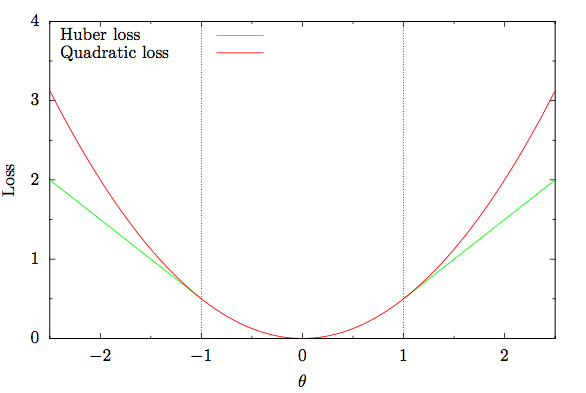
\includegraphics[height=80mm, width=100mm, scale=0.5]{chapters/huber.png}
\centering
\caption{Huber and squared loss}
\label{fig:s2} 
\end{figure}
\item \textbf{Kaiming initialization}: a method for weights matrix initialization, described in \cite{kaiming}, which draws samples from a standard normal distribution, to avoid \textbf{vanishing} and \textbf{exploding gradient}, and then adjusts this distribution to the ReLU activation function, by doubling the variance, since ReLU halves it w.r.t. to the original standard normal distribution (see \ref{fig:s3}).
\begin{figure}[H] 
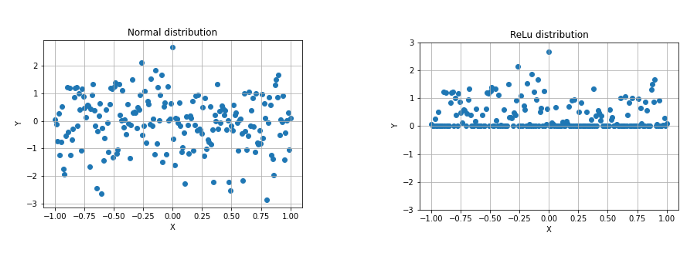
\includegraphics[height=80mm, width=140mm, scale=0.5]{chapters/relu_dist.png}
\centering
\caption{Normal and ReLU distributions}
\label{fig:s3} 
\end{figure}
\end{itemize}

\subsection{Dueling}

The model was further improved with \textbf{dueling} architecture. The main issue of standard DQN lies in the fact that the \textbf{Bellman operator} tends to overestimate the Q value: as stated in \cite{dueling}, the solution seems to be to separate the computation of the Q value in 2 separate functions, $$Q_{\pi}(s,a) = V_{\pi}(s) + A_{\pi}(s,a) $$ The \textbf{advantage} $A(s,a)$, which computes the  ''advantage'' of taking the action a in state s w.r.t. the other possible actions in that state, and the \textbf{value} $V(s)$ which simply measures how good the state s is, regardless of the possible actions; this is particularly useful whenever we're dealing with environments that are not affected by actions in every state, like Flatland, where actions are only really relevant at switches.

\begin{figure}[H] 
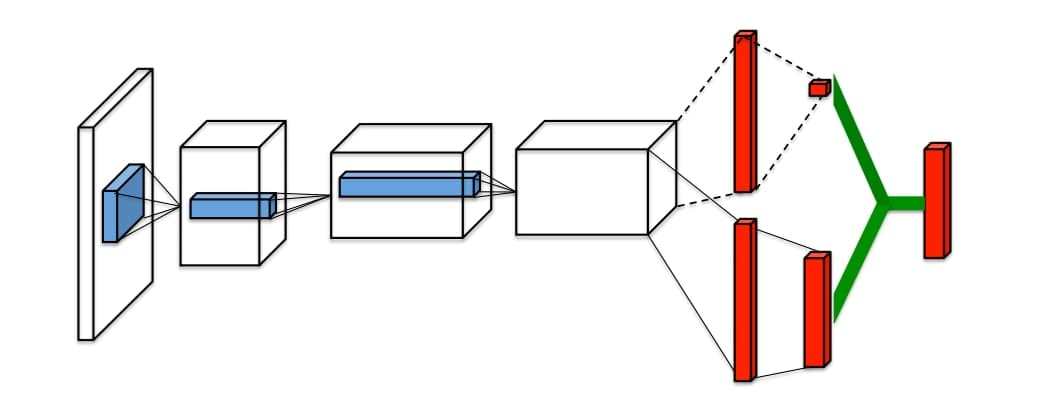
\includegraphics[height=80mm, width=140mm, scale=0.5]{chapters/dueling.jpg}
\centering
\caption{Dueling DQN}
\label{fig:s4} 
\end{figure}
\noindent
Advantage and value still need to be recombined, and since the standard formula doesn't allow to extract A and V from the Q value, \cite{dueling} suggested to force the advantage to be 0 at the chosen best action, which results in the output formula for Q $$Q_{\pi}(s,a) = V_{\pi}(s) + (A_{\pi}(s,a) - max_{a' in A} A(s,a'))$$ It also highlights, however, that empirically, subtracting the average advantage yields better results.
